\setchapterimage[6.5cm]{icecube}
\setchapterpreamble[u]{\margintoc}
\chapter{IceCube Neutrino Observatory}
\labch{icecube}
\begin{fquote}[Edmund Hillary][][1957] I am hell-bent for the South Pole — God willing and crevasses permitting.
\end{fquote}
The IceCube Neutrino Observatory is the world's largest neutrino telescope, located at the geographic south pole. It was built as a successor to the AMANDA experiment, which had pioneered the detection of neutrinos in ice. AMANDA served as a proof of concept for the detection of neutrinos, but with a volume of just nkm$^{3}$, it only had sufficient effective area to measure atmospheric neutrinos. 

IceCube, on the other hand, was envisioned as a much larger detector capable of measuring astrophysical neutrinos. It was constructed in phases from 2006 to 2011, eventually reaching a total volume of one cubic kilometer. The following sections detail the functioning of the IceCube detector.

\section{The IceCube Detector}

IceCube is composed of 86 strings arranged in a hexagonal grid \sidecite{icecube_detector_17}. Each string is 2.5 km long, and carries 60 regularly-spaced Digital Optical Modules (DOMs) containing Photo-Multiplier Tubes (PMTs). With a hot-water drill, holes were drilled into the glacier ice to a depth of 2.5 km. After string deployment, the liquid-filled holes refroze, fixing the DOMs in place. In total, there are 5160 DOMs deployed in IceCube, all at depths greater than 1km. The Antartic ice itself thus provides the detection medium for neutrinos, with the Earth acting as a shield against atmospheric muons. Data processing occurs at the \emph{IceCube Lab} (ICL), a dedicated building in the center of the detector. The full dectector can be seen in Figure \ref{fig:ic_detector}.

\begin{figure}
	\centering 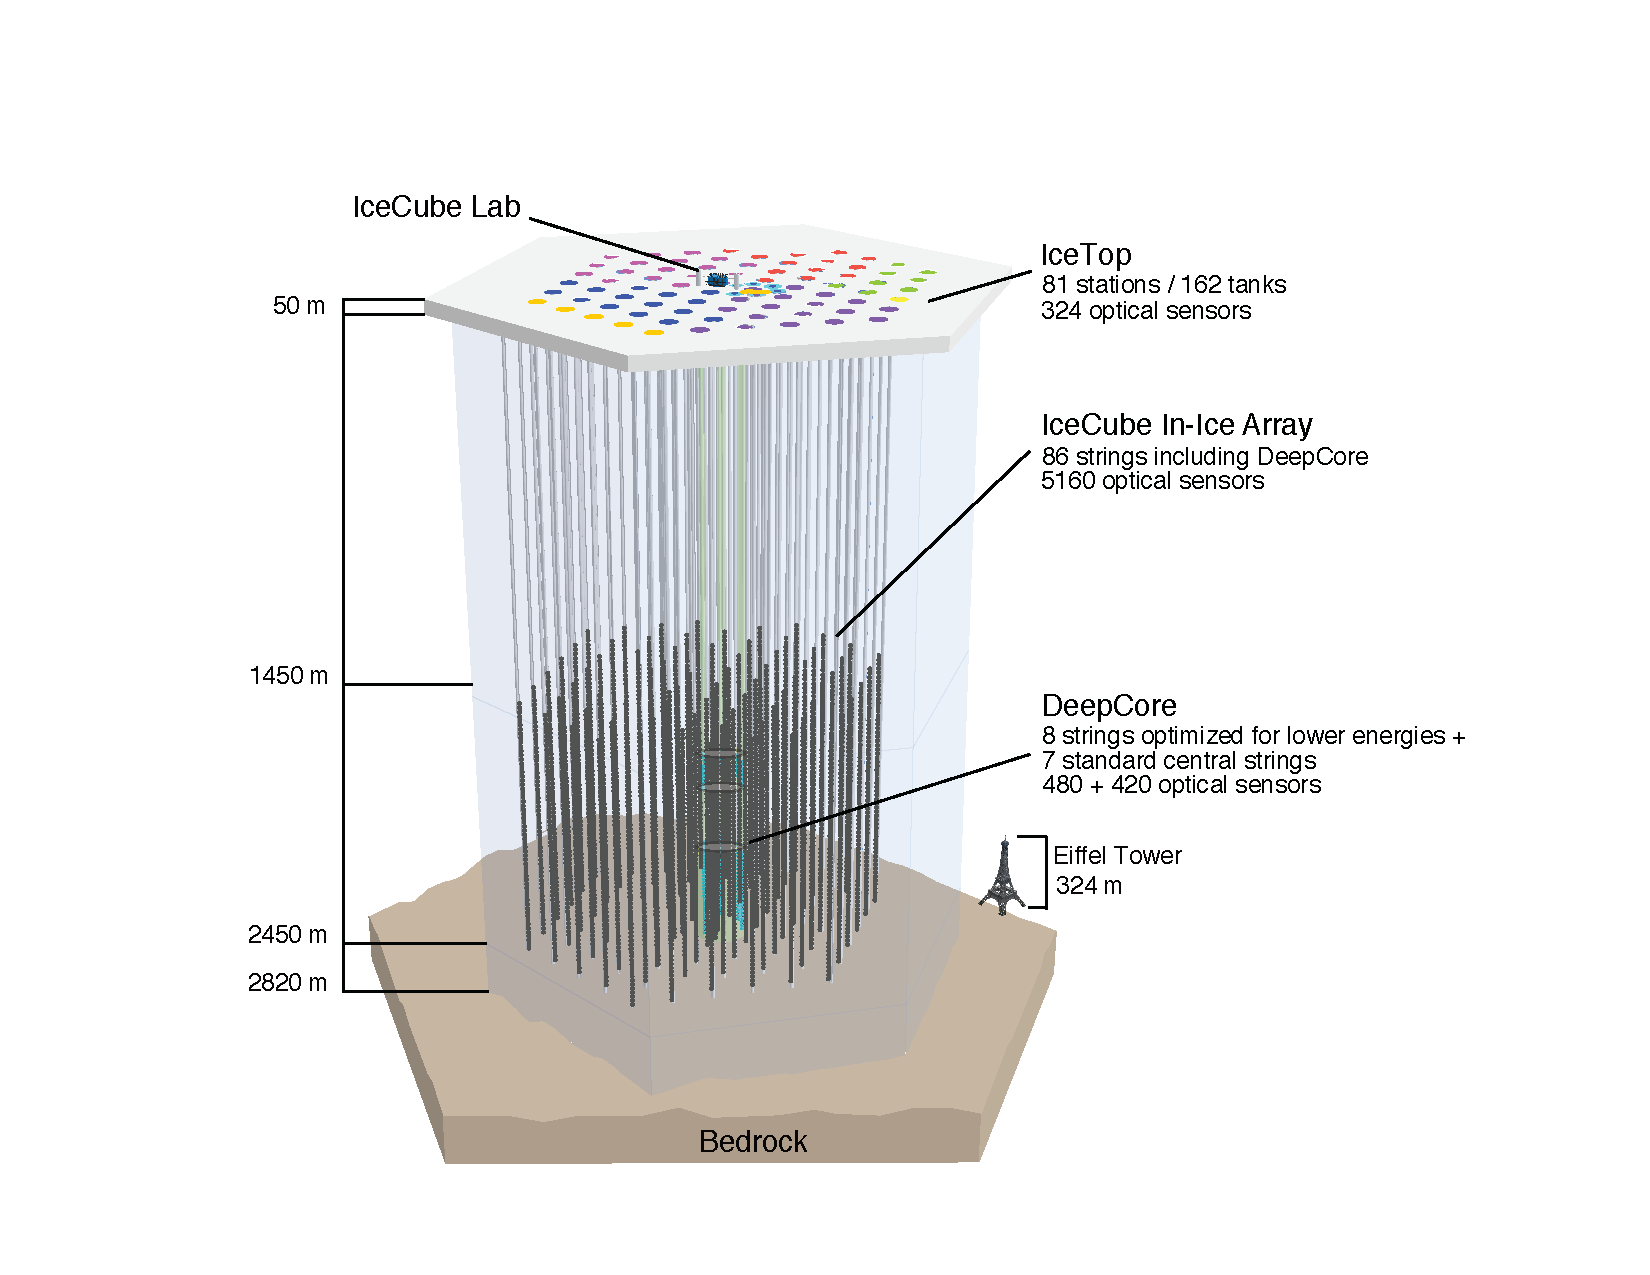
\includegraphics{icecube/ArrayWSeasonsLabels_crop}
	\caption{An overview of the IceCube detector, from \cite{icecube_detector_17}.}
	\label{fig:ic_detector}
\end{figure}

\subsection*{DeepCore}

The design of IceCube is an optimisation trading DOM-density against effective area for fixed cost. A minimal DOM density is needed to identify and reconstruct an event, and this threshold decreases as neutrino energy increases. Thus, while IceCube is generally optimised for detecting high-energy neutrinos in the astrophysical regime, it is far too sparse to effectively measure lower-energy (1-100 GeV) neutrinos. Therefor, in addition to the regular grid of strings, IceCube contains a denser in-fill array known as \emph{DeepCore}. This array consists of 8 dedicated strings and 7 standard strings, totalling 900 DOMs, and typically uses the outer IceCube detector as a veto against muons?. \textit{Deepcore} measures low-energy neutrinos which form the basis of neutrino oscillation studies, but can also be used for neutrino astronomy at lower energy scales.

\subsection*{IceTop}

IceCube also contains a surface array of instrumented ice tanks known as IceTop, which are used to measure surface air showers arising from cosmic rays and photon interactions. IceTop can be used as a veto against muons from air showers, but only for a small fraction of events which are almost-vertically down-going. However, IceTop also functions in its own right as a Cosmic-Ray detector, and contributes competitive measurements of the cosmic ray flux and composition.

\section{Neutrino Signals in IceCube}
\label{sec:nu_signal}

Neutrinos are indirectly detected in IceCube via charged secondary particles produced through interactions in the ice. These daughter particles, arising from both \emph{charged-current} (CC) and \emph{neutral current} (NC) interactions, emit via the Cherenkov effect when travelling faster than the local speed of light in ice. The light is emitted at a characteristic Cherenkov Angle, $\theta_{c}$, determined by the refractive index in ice and the particle velocity:

\begin{equation}
	\theta_{c} =  \arccos \left( \frac{1}{\eta \beta} \right)
\end{equation}

These Cherenkov photons travel through the ice, and can then be detected by one or more DOMs. During propagation, these photons can be both scattered or absorbed by the ice, which is somewhat inhomogeneous. In particular, there is a substantial layer of dust spanning the central depth range of the detector, and scattering is consequently elevated in this region. In general, the light emission serves as an excellent proxy for energy deposited in the detector, such that IceCube can reconstruct deposited energy with a resolution of $\sim$15\% \sidecite{ic_energy_reco_14}. 

\begin{figure}
	\centering 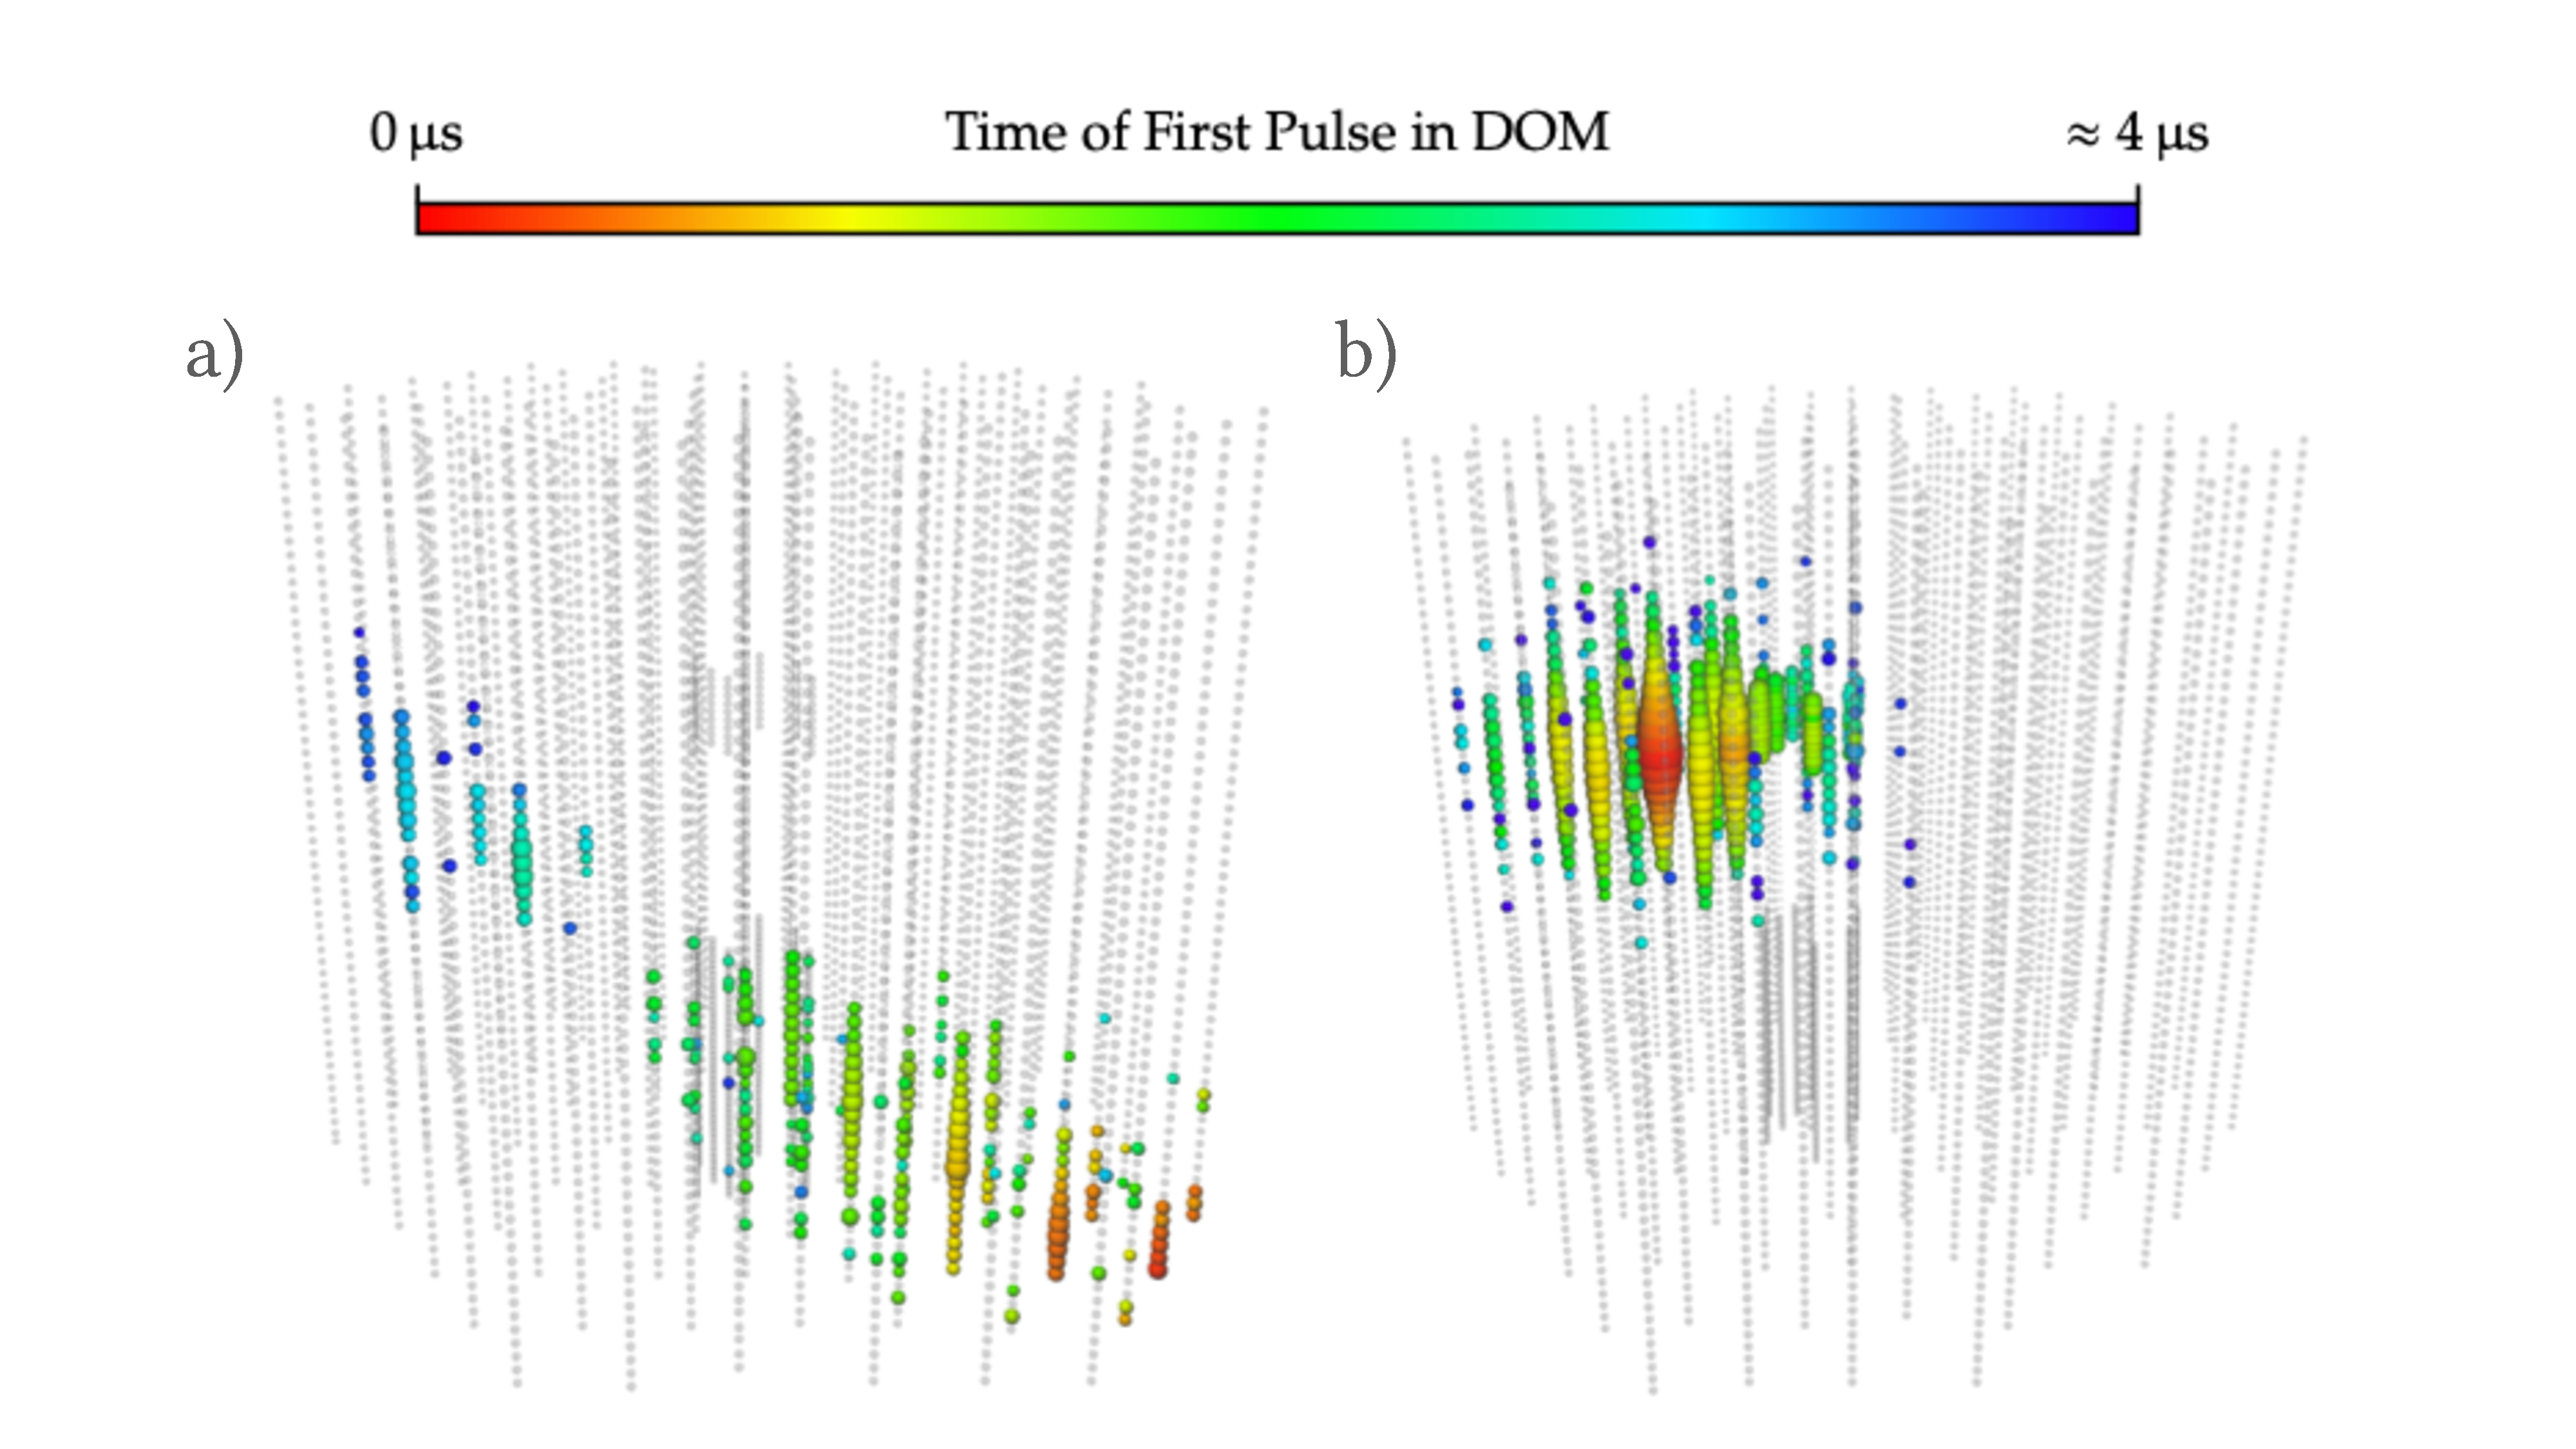
\includegraphics{icecube/event_view_a}
	\caption{Neutrino interaction signatures in IceCube, from \cite{kintscher_thesis}.}
	\label{fig:event_views}
\end{figure}

Different classes of physical interactions also produce different patterns of light deposition in the detector. There are two standard event topologies that IceCube detects from astrophysical neutrinos, namely \emph{Tracks} and \emph{Cascades}. These are illustrated in panel (a) and (b) of Figure \ref{fig:event_views} respectively \sidecite{kintscher_thesis}, where each sphere represents a DOM, the sphere radius is proportional to deposited charge and the colour represents the temporal evolution of the light deposition from early (red) to late (blue). 

Tracks arise from CC $\nu_{\mu}$ interactions, which produce daughter muons that typically traverses the detector while ionising the ice. Such \emph{through-going tracks} typically have well-reconstructed $\sim$1 \arcdeg-resolution directions, because the kilometer-scale lever arm can constrain the muon trajectory well. However, by virtue of the muon having lost an unknown energy fraction prior to entering the detector, these events typically have very poor energy resolution of .... The example through-going track shown in panel (a) of Figure \ref{fig:event_views} is, in this case, moving upwards through the detector (an \emph{upgoing track}), but \emph{horizontal track} and \emph{downgoing track} topologies are also possible. 

A small subset of events are \emph{starting tracks}, for which the CC $\nu_{\mu}$ interaction occurs within the detector. In such events, a roughly-speherical particle \emph{cacade} is generated at the interaction vertex, as well as an outgoing track from the daughter muon leaving the detector. For these starting tracks, energy resolution is improved but directional reconstruction accuracy can be degraded due to the shorter lever arm. Neutrino astronomy primarily relies on the use of both through-going and starting track events, and thus these are most relevant for this thesis. 

For charged-current electron neutrino interactions, the daughter electron will almost immediately generate an \emph{electromagetic cascade}, resulting in a near-spherical cascade signature without accompanying outgoing track \sidecite{spurio_18}. One such event is shown in Figure \ref{fig:event_views}. For cascades, nearly-spherical light emission results in a poor angular resolution of order 10 degrees. However, as the light is typically fully contained by the detector, IceCube can act as a calorimeter and constrain the neutrino energy with a resolution of $\sim$15\%. 

Neutral-current interactions of all flavours produce similar cascade-like signatures from \emph{hadronic particle showers}, consisting of.... Both cascade classes appear identical within the resolution of IceCube. Unlike $\nu_{e}$ CC interactions, for which the deposited energy corresponds to the incoming neutrino energy, NC interactions have an outgoing neutrino carrying a fraction of the charge. Additionally, hadronic showers have $\sim$15\% lower light yield because a fraction of the energy carried by electrically-neutral particles which are effectively invisible \cite{ic_energy_reco_14}. NC cacades thus have considerably more uncertainty on incoming neutrino energy \cite{ic_energy_reco_14}.

Charged-current $\nu_{\tau}$ interactions lead to the production of a tau with various possible signatures. As with other CC interactions, a ?? cascade is generated at the primary interaction vertex. In $\sim$17\% of interactions, the tau will decay to a muon, yielding an outgoing track signature. Alternatively, the tau will propagates through the ice before decaying to an electron. in which case a second cascade is produced. The latter is a unique tau topology, known as a \emph{Double-Bang}. The separation between these cascades, $L_{DC}$ will vary depending on the degree of length contraction experienced for the tau before decay, and is thus roughly proportional to energy:

\begin{equation}
	L_{DC}  \approx \frac{E_{\nu_{\tau}}}{\textup{1 PeV}} \times 50 \textup{m}
\end{equation}

Given the vertical  DOM spacing in IceCube of $\sim $17 m, a minimal tau energy of approximately $\sim$100 TeV is required for such events to be identified. IceCube has reported the probable detection of two such Double-Bang $\nu_{\tau}$ events, though dedicated waveform analysis was required to distinguish emission from the two cascades \sidecite{Stachurska_thesis}. 

\section{Atmospheric Backgrounds in IceCube}

The IceCube detector geometry is non-isotropic, and this leads to a zenith-dependence in both effective area and background rate. In addition, for higher energies above $\sim$100 TeV, Earth absorption increasingly suppresses upgpoing neutrino events. Event selections are designed to balance signal acceptance rate and atmospheric background contamination, typically acheived for neutrino astronomy selections by optimising for final analysis sensitivity as a function of detector zenith (see Chapter \ref{sec:llh}). 

There are multiple classes of atmospheric background that can masquarade as track-like signatures used for this thesis. Atmospheric air showers provide the dominant source of background events in the detector, with daughter \emph{atmospheric muons} frequently having sufficient energies to penetrate the 1 km ice overburden and reach the IceCube detector. These atmospheric muons only produce downgoing tracks, because horizontal and upward-going events are effectively suppressed through muon-shielding from the Earth. In addition, cosmic ray air showers produce an isotropic flux of \emph{atmospheric neutrinos}, which are not shielded by the Earth. There is thus an isotropic atmospheric neutrino background, and an additional atmospheric muon background for southern declinations of the sky. The atmospheric neutrinos are indistinguishable from astrophysical neutrinos at an individual event level, and are detected at a substantially larger rate except at the very highest energies, as can be seen in Figure X!!!!!!!

\begin{figure}
	\centering 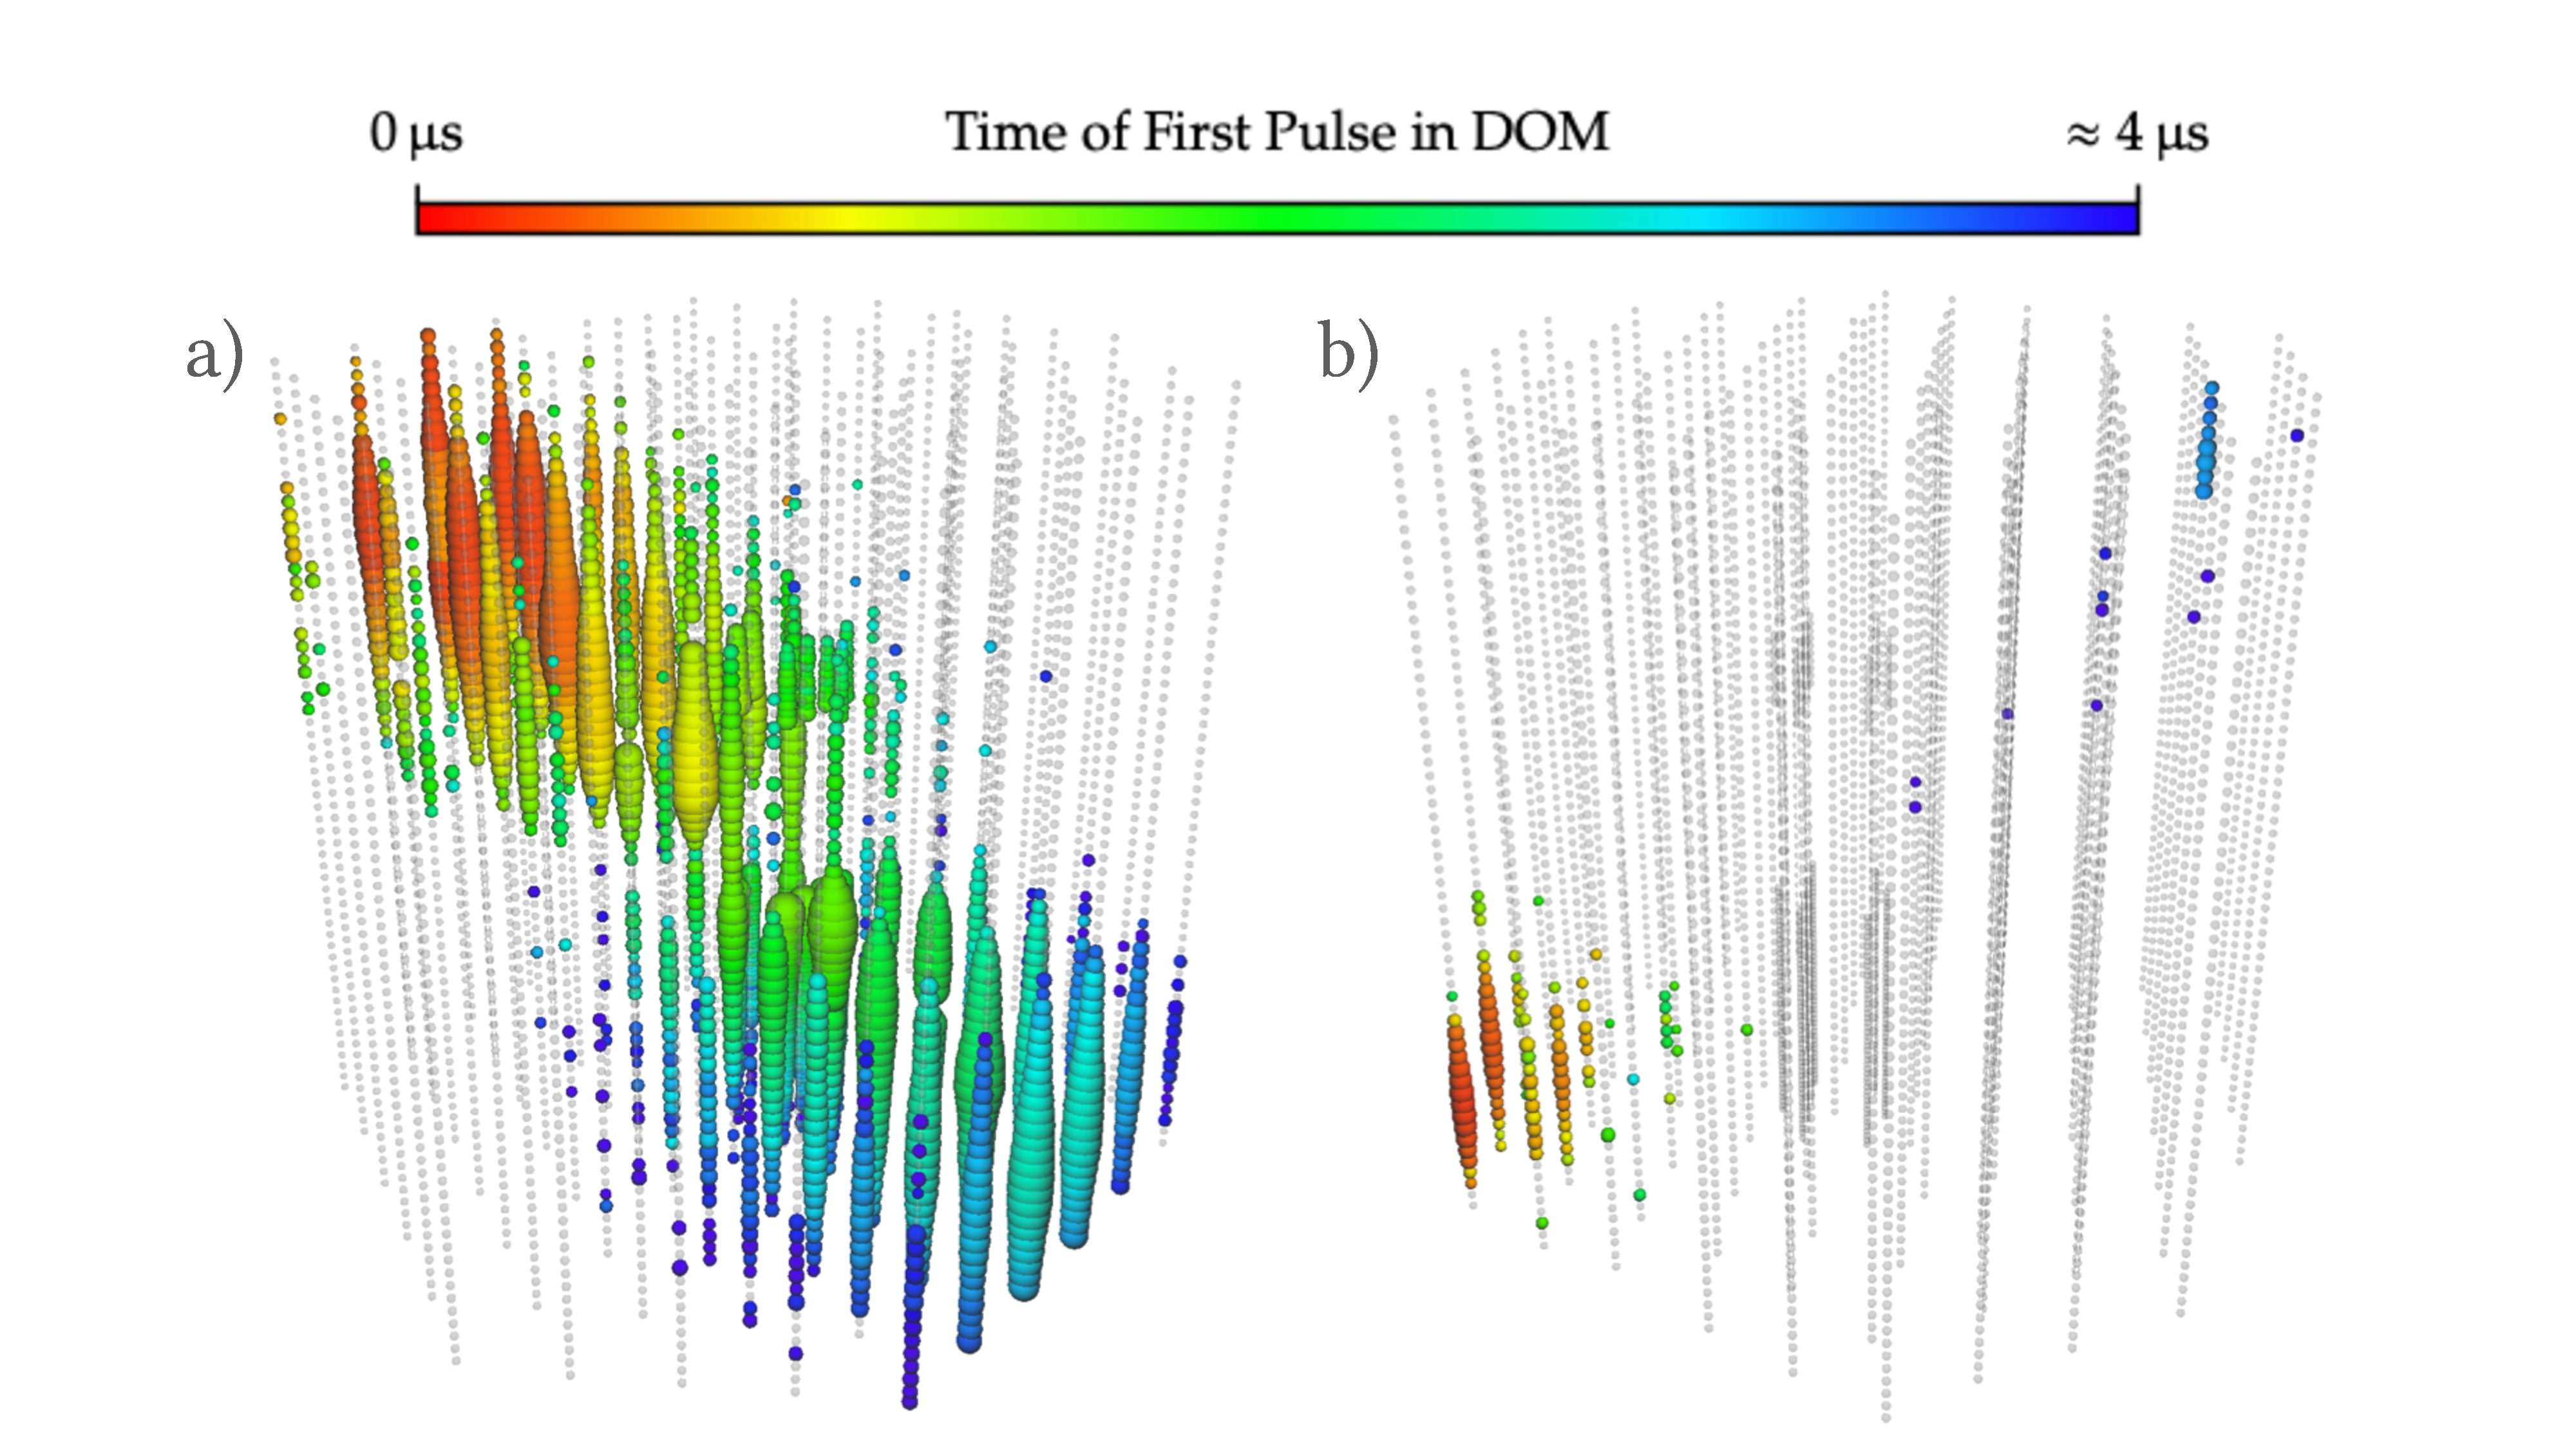
\includegraphics{icecube/event_view_b}
	\caption{Examples of atmospheric muon background signatures, from \cite{kintscher_thesis}.}
	\label{fig:event_views_bkg}
\end{figure}

To reject the overwhelming muon background, downgoing track selections typically include strict energy cuts to reject atmospheric muons below $\sim$10 TeV. Above these energies, indivudual muons of atmospheric origin are unlikely. However, multiple daughter muons can travel as a \emph{muon bundle}, which within the resolution of IceCube might appear to be one single high-energy muon. Panel (a) of Figure \ref{fig:event_views_bkg} illustrates one such muon bundle containing many muons produced from an air shower arriving above the detector. Often cascade-based downgoing analyses have superior sensitivity to muon-track based ones as a result of the improved energy resolution and suppressed muon-bundle background, because energy-based discrimination is ultimately the most effective method to distinguish signal from background in such cases.

Upgoing event selections can typically probe lower-energies as a result of the reduced atmospheric muon background, though in addition to the atmospheric neutrino background these selections also suffer from some residual muon contamination. Panel (b) of Figure \ref{fig:event_views_bkg} illustrates one example involving two \emph{coincident atmospheric muons} which can trick trigger algorithms.

% but upgoing fluxes with a large chord length through the Earth are suppressed through absorption. Consequently IceCube reaches peak sensitivity for horizontal events, which benefit from both high background rejection and low earth absorption. It is in this region that the highest-energy track-like events at $>$200 TeV are typically found. 

For sufficiently high-energies, the low opacity to muons from air showers means that any atmospheric background event is very likely to be accompanied by additional and near-simultaneous muons from the same air shower. By rejecting so-called \emph{coincident events} with multiple particles inside the detector, the \emph{self veto} becomes an effective method to reject southern-sky background at energies beyond nTeV. This significantly improves on air-shower rejection using the IceTop detector, which is only effective for near-vertical downgoing events.

Another effective method to reject background muons is to focus solely on \emph{starting events}, aiming to identify cases where the interaction vertex lies well within the detector CITEHESE. Using outer detector layers as a selection veto reduces effective volume, but for such cases, almost all atmospheric muon backgrounds are rejected. 

\section{Digital Optical Modules (DOMs)}

\begin{marginfigure}
	\centering 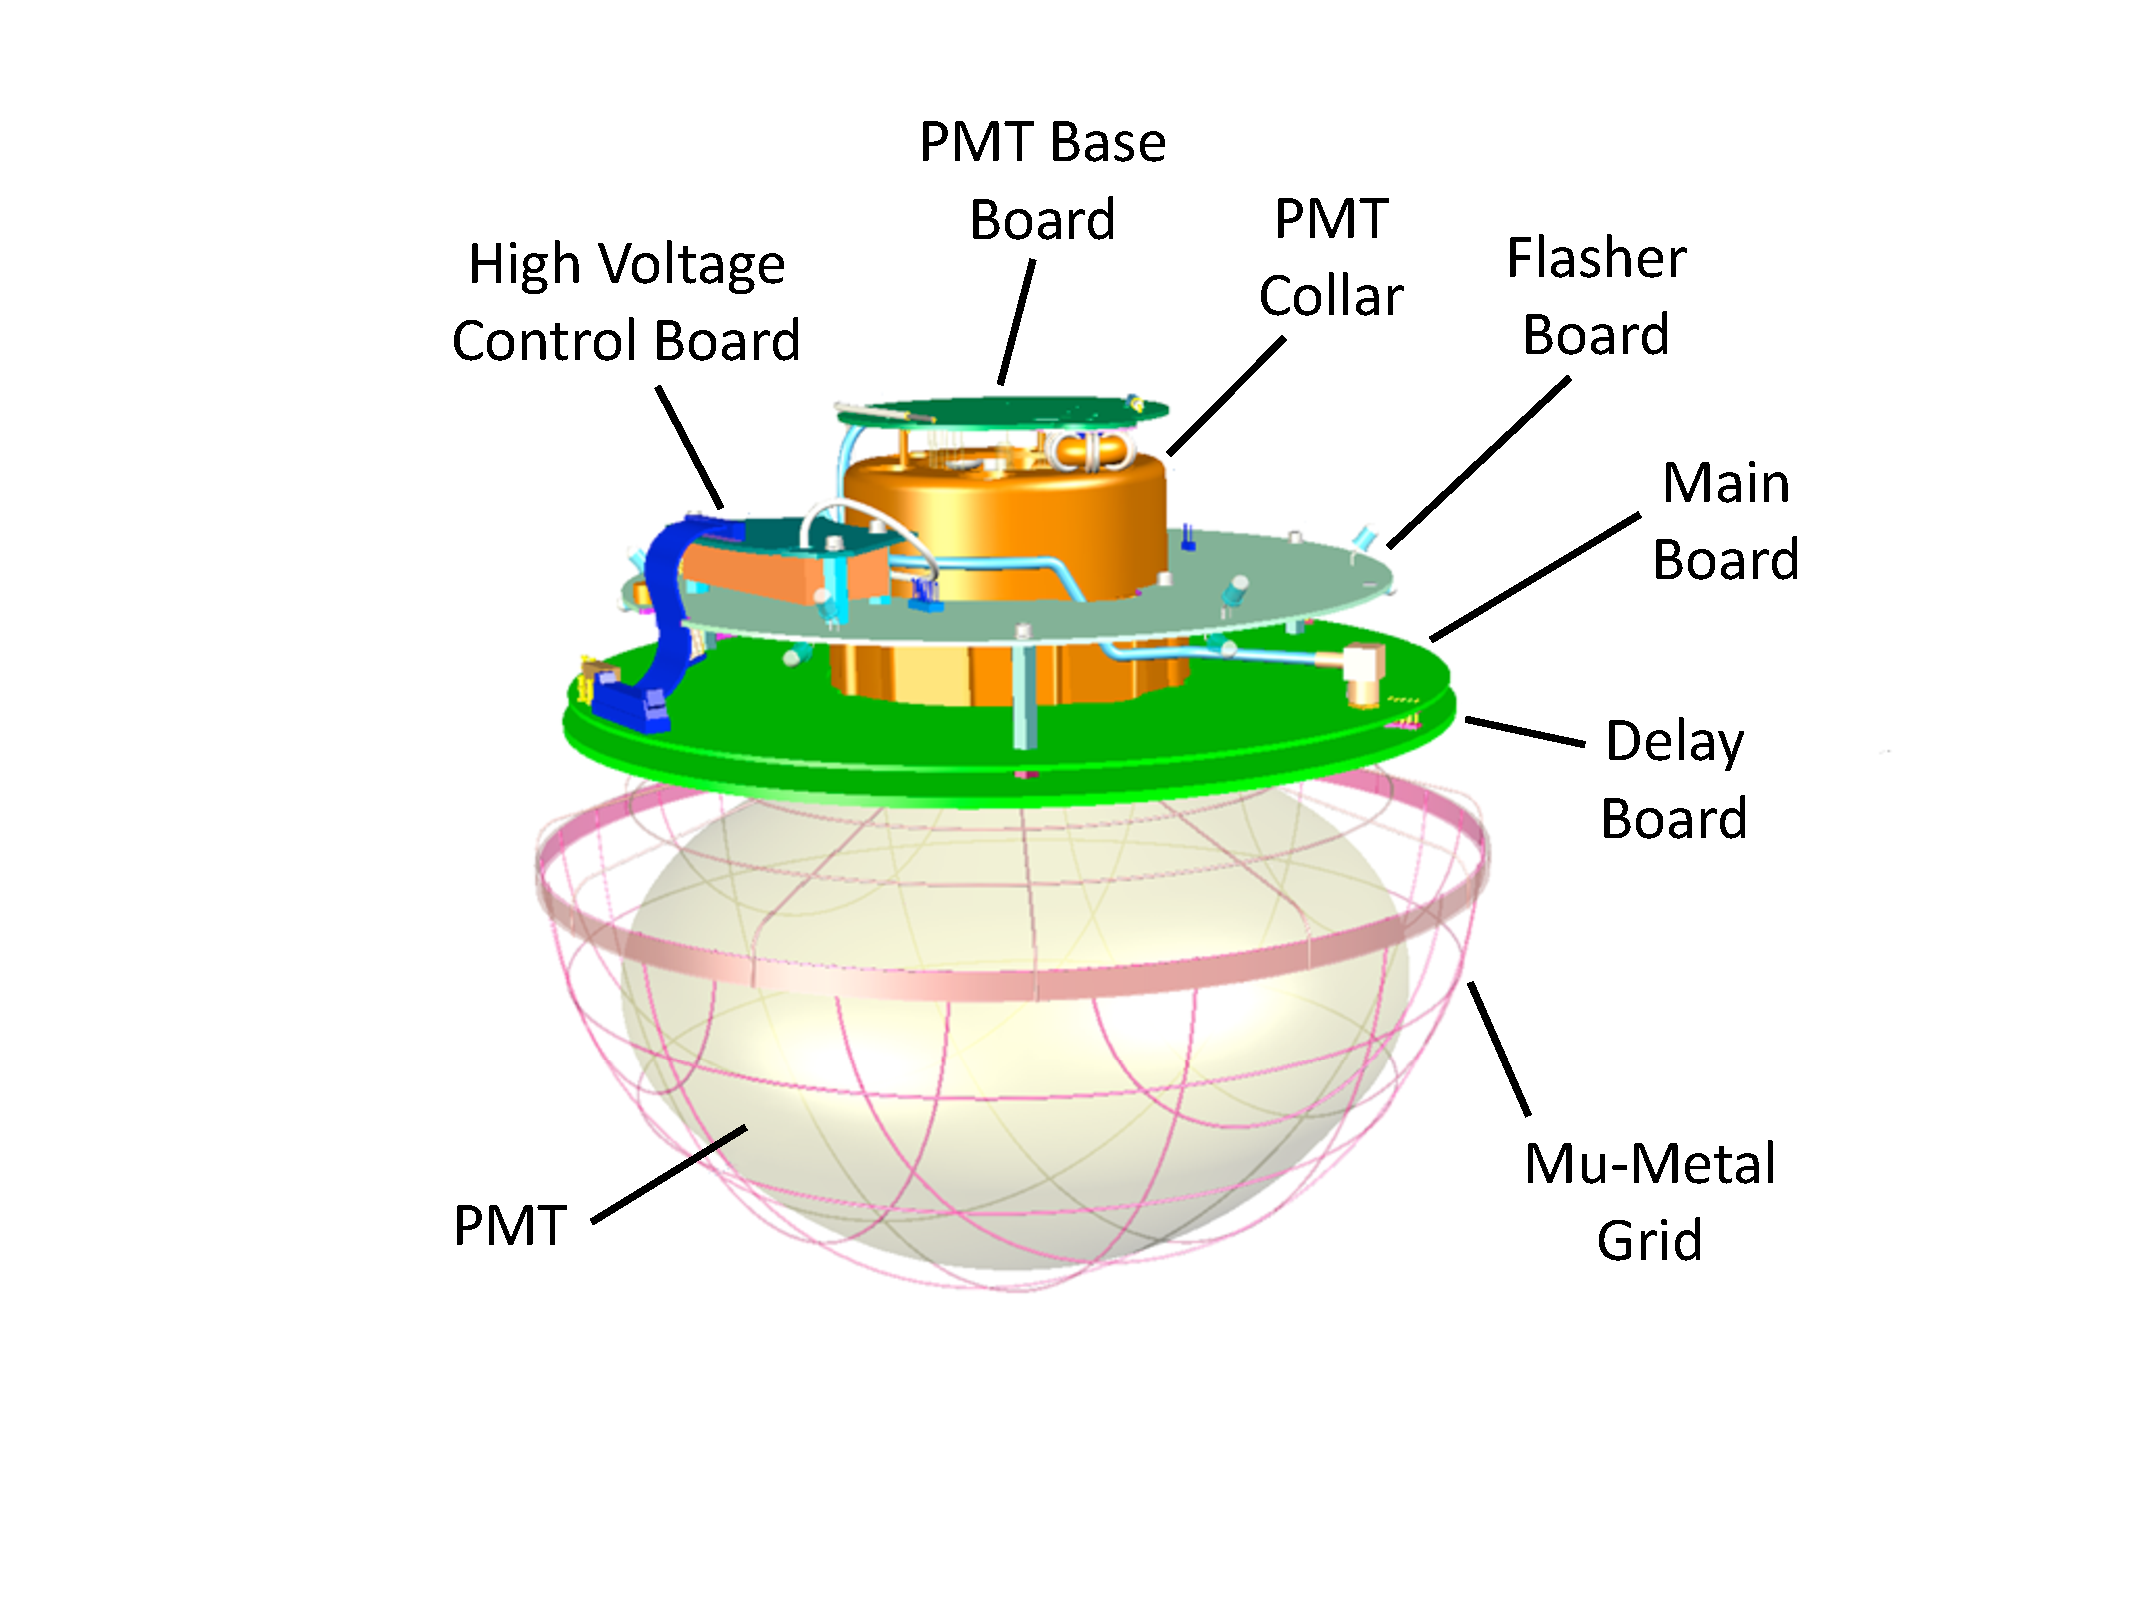
\includegraphics{icecube/domfig1a-DOM3DModel}
	\caption{An overview of an IceCube DOM, from \cite{icecube_detector_17}.}
	\label{fig:dom}
\end{marginfigure} 

The process of actually detecting neutrino interactions in IceCube begins with the detection of individual photons using \emph{Digital Optical Modules} (DOMs). Each DOM contains a single downward-facing PMT encased in a glass sphere to withstand glacier pressure, along with a main board containing electronic readout systems. DOMs also contain \emph{flashers}, which are sets of LEDs used for calibration purposes including DOM timing precision, position and to infer ice optical properties. The major DOM components can be seen in Figure \ref{fig:dom}. Each DOM is connected via cabling directly to the ICL, but also to neighbouring DOMs on the same string via dedicated \emph{local coincidence} wiring as seen in Figure \ref{fig:dom_cable} \cite{icecube_detector_17}.

\begin{marginfigure}
	\centering 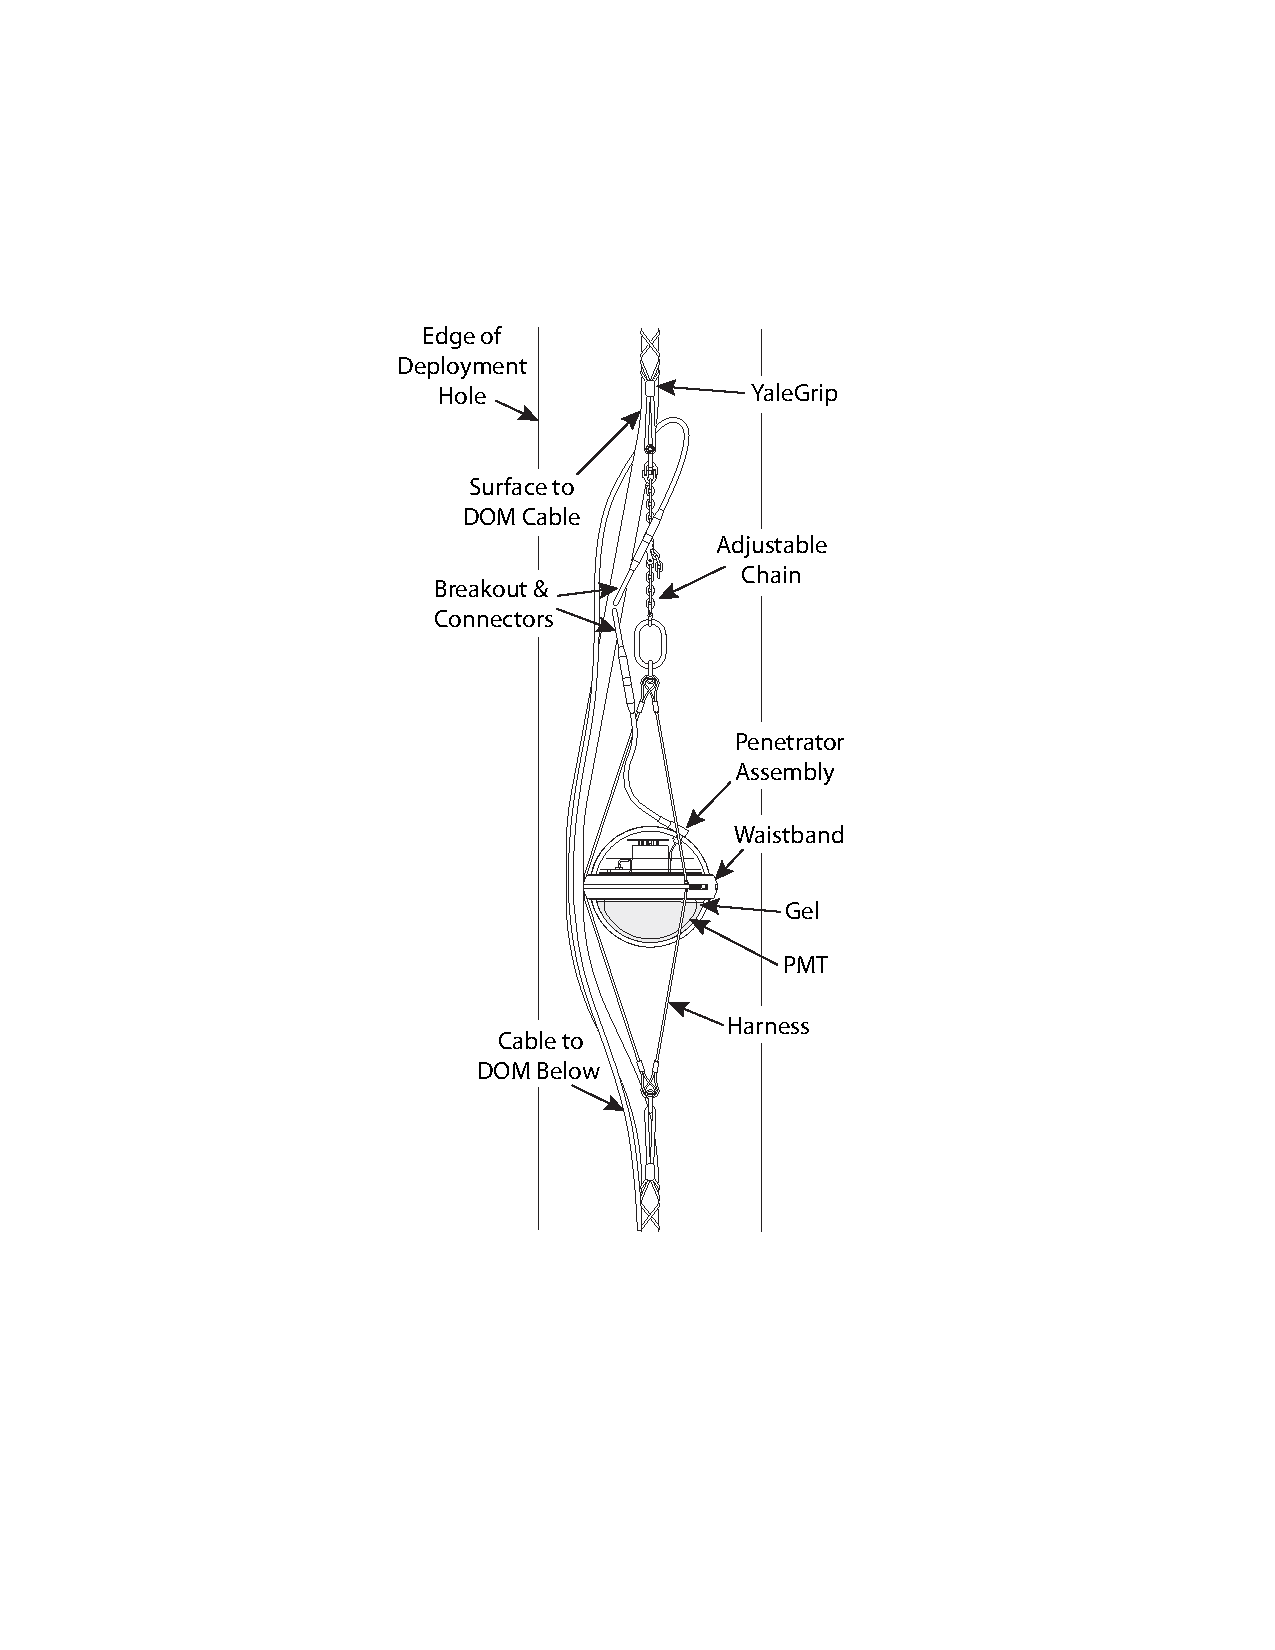
\includegraphics{icecube/domfig2a-CableAssembly}
	\caption{DOM cabling structure, from \cite{icecube_detector_17}.}
	\label{fig:dom_cable}
\end{marginfigure} 

\subsection*{Photomultiplier Tube (PMT)}

IceCube is ultimately a photon detector, relying on the Photomultiplier Tubes (PMTs) to collect data on the light emission associated with neutrino interactions. PMTs rely on the \emph{photoelectric effect} introduced in Chapter \ref{ch:nu_theory}, with individual photons ioning single atoms in a \emph{photocathode}, releasing single electrons. In a PMT, a high voltage is applied to accelerate these liberated electrons, ideally resulting in an amplified signal which can ultimately be detected. Icecube PMTs have a \emph{gain} (amplification ratio) of 10$^{7}$ and reach a peak \emph{Quantum Efficiency} (QE) of $\sim$25\% at 390nm, i.e one in four photo-electrons reaching the PMT are then detected. 

The glass itself has a high 93\% optical transmission at 400nm, while the PMT sits in a silicon gel with optical transmission of 97\% at 400nm, with good optical coupling that results in <0.1\% reflectivity from glass to gel to PMT \cite{icecube_detector_17}. 

\subsection*{Mu-Metal Grid}

The South Pole magnetic field would be sufficiently strong to impact PMT performance, with 550mG collection efficiency ultimately reduced by 5-10\% and gain variations of 20\% depending on azimuth orientation \cite{icecube_detector_17}. To mitigate this effect, each DOM has a dedicated shielding structure. This consists of a wire mesh constructed from \emph{mu-metal}, an alloy with high magnetic permeability, which results in a collection efficiency reduction of <2\% \cite{icecube_detector_17}. 

\subsection*{Waveform Capture}

Signals in each PMT are compared to a discriminator threshold of 0.25 photoelectrons (PE), above which the process of \emph{waveform capture and digitisation} is triggered. DOMs have both an \emph{Analogue Transient Waveform Digitiser} (ATWD)  and a \emph{fast Analogue Digital Converter} (fADC) for this process. ATWDs will record for 427ns, sufficient to cover light with 10s od meters of a DOM, while fADCs operate continuously with a lower sampling rate to record the longer signals. Each ATWD has three channels with different gains, to ensure that no information is ever lost to saturation. If there are local (neighbour or next-to-neighbour) coincident hits, they are classified as \emph{Hard Local Coincidence} (HLC) hits and the full waveform is compressed and sent to ICL. For isolated \emph{Soft Local Coincidence} hits only a summary is sent.

\section{Data Processing}

While the individual hits in DOMs are dominated by dark noise, HLC hits are generally dominated by `real' detections of atmospheric muons with a rate of $\sim$2.5-2.9 kHz \cite{icecube_detector_17}. All HLC hits are read out, combined with contemporaneous HLC hits from other DOMs, and filtered. There is an initial raw data rate of 1Tb/day. 

There are several iterative steps for data processing, with limited computing resources and transfer bandwidth at pole necessatiating a multi-step filtering process. Only low-resource calculations can be applied at pole. Data is then transferred via satellite to dedicated computing reasources in Madison, WI, where more advanced calculations are then applied.

For this thesis, the relevant base filter is the \emph{muon filter}, which selects HLC hits that are consistent with a muon track hypothesis. Multiple final-level filter chains were utilised in this thesis to cover different data-taking periods, as introduced in Chapter \ref{ch:results}, but all track selections follow a similar process. For the \emph{GFU event selection} \cite{kintscher_thesis} (utilised for the analysis of AT2018cow in Chapter \ref{ch:results}) the following steps were applied:

\begin{itemize}
	\item \textbf{Simple Multiplicity Trigger}- Events are initially selected based on a threshold number of HLC hits within a sliding time window \cite{icecube_detector_17}. For the muon filter, the relevant trigger is SMT-8, where $\geq$8 hits are required to occur within 5$\mu$s.
	\item per-DOM response used to unfold light arrival time and amplitude
	\item \textbf{Application of online reconstruction algorithms} - The simple track trajectory reconstruction known as \emph{LineFit} is applied to events (see Section \ref{sec:reco}).
	\item \textbf{Application of the muon filter} - The \emph{muon filter} selects track-like events using the likelihood value from LineFit to assess the compatability of the data with a muon track hypothesis, removing unwanted cascade events. There are additional cuts on cumulative charge for down-going events, yielding a combined passing rate of 40 Hz \cite{kintscher_thesis}.
	\item \textbf{Transfer filtered data via satellite } - Events passing one or more online filters are transferred via satellite connection to Madison, yielding a combined data rate of $\sim$90 Gb/day for all filters.
	\item \textbf{Application of further reconstruction algorithms} - A selection of more demanding direction and energy reconstructions are applied (see Section \ref{sec:reco}).
	\item \textbf{Application of the OnlineL2 filter} - Relying on the outcome additional reconstructions, the \emph{Online Level 2 filter} (OnlineL2) applies additional algoithmic cuts on charge, reconstructed track length, number of hits and log likelihood values to select high-quality tracks with a combined passing rate of $\sim$5 Hz \sidecite{voge_thesis}.	
	\item \textbf{Application of the GFU filter} - The final-level event selection consists of both algorithmic cuts and the application of a dedicated \emph{Boosted Decision Tree} (BDT) to select well-reconstructed high-quality tracks for use in likelihoood analysis (see Chapter \ref{ch:llh}), with a final event rate of 6.5 mHz \cite{kintscher_thesis}.
	\item \textbf{Application of the Realtime alert filter} - Additional filter to identify exceptional high-energy events with a high probability of an astrophysical origin, which are then immediately published via the NASA Gamma-ray Coordination Network (GCN) \sidecite{ic_realtime_19}. These realtime events have additional time-consuming reconstruction algorithms applied (see Chapter \ref{ch:realtime}), with an overall trigger rate of $\sim$1 event per two weeks.
\end{itemize}

\section{Event Reconstruction}
\label{sec:reco}

The arrival time of event is known with ns-scale????????? precision due to robust DOM time calibration, a level at which timinig uncertainty is negligible for all neutrino astronomy analysis. There are then two main observables that must be reconstructed for the neutrino astronomy analysis in Chapter \ref{ch:llh}, namely the incoming neutrino energy and incoming neutrino arrival direction. The uncertainty on both these reconstructed quantities can be derived from Monte Carlo simulations based on similar events, but the angular error estimates also utilises properties of the direction reconstruction likelihood landscape (see Section \ref{sec:pull correction}). In the standard reconstruction chain, robust but simplistic algorithms are often employed in order to generate a seed for minimsation in more complex reconstructions. The seeding approach ensures stability and speed. 

\subsection{Track Reconstructions}

\subsubsection*{LineFit}
The \emph{LineFit} algorithm is the most simplistic approach to reconstructing a muon track, based on the assumption of a uniform cylinder of light traversing the detector at a constant speed \sidecite{ic_track_14}. The arrival time of photons $t_{i}$ at each hit DOM, defined as the time of detection of the first photo-electron, is combined with the spatial position of each DOM, $\vec{x_{i}}$, and the residual squared distance from signal hypothesis is then evaluated:

\begin{equation}
	\sum^{N}_{i} d_{i}^{2}(t_{0}, \vec{x_{0}}, \vec{v})= \sum^{N}_{i}  \left( \vec{v}(t_{i} - t_{0}) - (\vec{x_{i}} - \vec{x_{0}}) \right)^{2}
\end{equation} 

where N is the number of hit DOMs, $t_{0}$ and $\vec{x_{0}}$ are the temporal and spatisl intersect of the track, and $\vec{v}$ is the track trajectory. LineFit thus only considers the position and first photoelectron arrival time of each hit (i.e each DOM), but does not utilise information about the charge distribution at each DOM. The three fit parameters $t_{0}$, $\vec{x_{0}}$ and $\vec{v}$ are optimised to minimise the residual squared distance. The result corresponds to a plane of light moving through the detector. Because of scattering and absorption, and the fact that the light is actually emitted in a conical shape, this direction only approximately follows that of the true muon direction. Nonetheless, the reconstruction simplicity makes it extremely robust, and thus forms the basis of most more-advanced reconstructions. 

\subsubsection{Single-Photon-Electron-fit (SPE fit)}

One step beyond a $\chi^{2}$ minimisation is to perform a full likelihood minimisation. In this case, if PDFs are constructed which accurately describe the physics in question, a more precise solution can be determined. The most simplistic model used in IceCube is the so-called \emph{Single Photon Electron} (SPE) likelihood. In this case, much like for LineFit, it is assumed that the first photon to arrive at a DOM is the one that is least scattered. This photon arrival time thus gives us the best indicator of the geometric distance the emitting muon.  A parameterised PDF is used to describethe scattering in ice, \cite{ic_track_14}. 

A PDF in constructed, across all DOMs, comparing the first detected photelectron in that DOM to that expected from a photon propagation model:

\[ L = stuff \]

\subsubsection{SplineMPE}
Assumption continuous energy losses
\subsubsection{Millipede}
Cascades

\subsection{Energy Reconstruction}

As mentioned in Section \ref{sec:nu_signal}, energy reconstructions primarily rely on the linear scaling of ligth with deposited energy. Reconstructing the muon neutrinos is more challenging bceause a significant fraction of the energy will be deposited outside the detector. In general, the muon energy in the detector can be estimated by measuring the energy deposition rate of the track, where average muon energy losses can be parameterised as:

\begin{equation}
	\frac{dE_{\mu}}{dx} = A + \left(B \times E_{\mu} \right)
\end{equation}

with A describing the fixed ioninisation energy losses and B describing additional stochastic energy losses due to e.g brehmstrahlung \sidecite{ic_truncated_energy_13}. Muons at $\sim$1 TeV are termed \emph{minimally-ionising muons}, which .... . Above this threshold,the stochasticity of energy deposition limits the resolution of reconstruction algorithms \cite{ic_energy_reco_14}. 

An essential component of energy reconstructions is the relation between deposited energy and light yield for the ice, which can be derived as a function of detector position and light orientation \cite{ic_energy_reco_14}. Detailed Monte Carlo simulations can be performed, including the detector response function an a model of the glacier ice, to derive this light scaling relation. Such simulation are prohibitively comuptationally expensive to be newly performed for individual events, so instead the results of simulations are stored in tabulated form, and interpolated through use of a \emph{spline function}. 

Having parameterised the light propagation, one of the reconstruction algorithms can then be used to reconstruct the muon energy. There are two relevant reconstructions used by event selections in this thesis:

\begin{itemize}
	\item \textbf{MuEX} - ...
	\item \textbf{Truncated Energy} - The track is divided into separate bins yielding multiple estimates of $\frac{dE}{dx}$, outlier energy depositions are discarded, and a mean rate of energy loss is calculated using the remaining bins. This process reduces the impact of large stochastic energy losses which would otherwise bias the total deposition estimate \cite{ic_truncated_energy_13}.
\end{itemize}

The resultant muon energy proxy estimates must also be corrected to estimate the neutrino energy at interaction, which may take place several kilometers away from the detector itself. Such energy corrections have substantial uncertainty, they are performed on an ensemble basis using Monte Carlo simulations.

\subsection{Angular Error estimation}
\section{Pull Corrections}
\label{sec:pull_correction}
In general, track reconstructions rely on reconstructing patterns of light emission from a muon traversing or exiting the detector. In that sense, they are more precisely muon track reconstruction algorithms. However, for the purposes of neutrino astronomy, we are instead interested in the neutrino direction. 

For neutrino interactions, the direction of the outgoing daughter lepton is random in the center-of-mass frame. Viewed from the detector frame, the leptons are preferentially emitted along the incoming neutrino trajectory, with a spread depending on interaction opening angle. This \emph{Kinematic Angle} between the neutrino and lepton is thus energy-dependent, with lower-energy neutrinos having on average larger opening angles. The Kinematic Angle $\theta_{k} $ can be approximately described as:


\begin{equation}
	\theta_{k} \approx 1 \arcdeg \times \frac{E_{\nu}}{\textup{1 TeV}}
\end{equation}

Given the poor cascade resolution, the Kinematic Angle is thus primarily relevant for muon tracks where the muon energy is below $\sim$10 TeV. This is however the parameter region in which the majority of the IceCube tracks fall, and is thus important to consider. The Kinematic Angle spread must be convoluted with the muon Point-Spread Function (PSF) in order to correctly model the expected distribution of tracks for a given neutrino source.

In an ideal case, this convolution would be done exactly. However, as discussed above, the neutrino energy for a given event can only be approximately determined. In practice, a correction must be performed based on the expected distribution of true neutrino energies corresponding to a given energy proxy value. Typically, this \emph{Pull Correction} is performed using weighted Monte Carlo events under the assumption a particular true energy neutrino distribution. In IceCube, it is traditional to assume an $E^{-2}$  spectrum. In any case, this step introduces a fundamental energy-dependence to the neutrino PSF, which will unavoidably be present for any neutrino telescope in this energy regime. 

\section{Detector Calibration}

\subsection{The polar ice}

dust layer, clear ice, scattering greater than absorption, calibrated using muons/flashers/laser


\section{Event signatures in IceCube}

cherenkov colour/wl

\subsection*{Flashers}
\subsection*{Moon Shadow}

DOMcal - once a year

Pedestal per run

DOM efficiency 10\%

calibrated with low-e muons (in energy reco paper)

Probs in other section 

dust layer volcano

DOMsn known 1m precision xyz



\section{SNDAQ}

While most event selections for GeV and TeV-PeV neutrinos require multiple DOM hits to reject thermal-noise background, a separate detection channel exists for MeV neutrinos that are typically produced in both stellar fusion and supernova collapse. These neutrinos form an irreducible background for the IceCbe detector, with extremely short track lengths that are only detectable by single DOMs. A dedicated SuperNova Data Aquistion System (SNDAQ) is installed to measure the rate of these single-DOM detections, and identify any significant deviation from expected rates. As demonstrated by SN1987a, any nearby supernova will produce a significant flux of MeV neutrinos during core collapse, and this will be manifested in a significant uptick in trigger rate that will evolve as a function of time. 

It is predicted that IceCube will be able to clearly measure the temporal evolution of MeV neutrinos from any supernova in the galaxy or Magellanic Clouds, similar to Figure NNNN. IceCube sends any mid-significance deviations from trigger rate to the SuperNova Early Warning System (SNEWS), where they are cross-correlated with other sensitive neutrino detectors such as SNO and Super-K. In the event of a multi-detector trigger, observatories around the world will be alerted to the upcoming optical counterpart of a galactic supernova, which can be localised in the case of a strong signal by combining directional information from individual detectors and time-delays between detectors in differing geographical locations. 

MeV neutrinos for supernovae.

\section{Proposed Improvements to the IceCube detector}

There are several planned or proposed extensions to IceCube that would substantially improve the detector performance. Beginning in 2023, deployment will start for the IceCube Upgrade, a Deepcore-like dense infill array. The string spacing will be even tigher than deepcore, with a higher density of DOMs. In combination with hardware improvements from multi-PMT DOMs, the Upgrade should push IceCube's lower energy threshold from a few GeV, and potentially to below one GeV. This opens up an entirely new regime for both oscillation studies and lower-energy neutrino astronomy relative to competitor neutrino detectors such as SuperK. In addition to the gains from DOMs, many new calibration devices will be deployed to more accurately constrain sources of systematic uncertainties, in particular the ice scattering and absorption length. With these calibration measurements, archival neutrino data can be reprocessed, providing more accurate reconstructed parameters. Improvement should be expected for all neutrino sources analyses, which all suffer to lesser or greater degree from these systematic errors. 

Beyond the IceCube Upgrade, a more comprehensive improvement is planned to extend the higher-energy capability of IceCube. IceCube-Gen2 is a proposed extension instrumenting 10 km$^{3}$ of ice, with a sparser string footprint than the existing detector. While multi-PMT DOMs should partially compensate the lower density, Gen2 represents a transition in focus to higher-energy neutrinos at 10TeV-100PeV range, at the cost of poorer resolution for lower-energy neutrinos with few DOM hits. Given the tenfold increase in instrumented volume, IceCube Gen2 will substantially increase sensitivity to both steady and time-dependent neutrino sources.

A further radio-based extension is proposed to complement the DOM-based Gen2 component. The detection of radio-based air shower detection has been demonstrated by the Pierre Auger Observatory, and its use in ice was pioneered by the ARA and ARIANNA collaborations. A pilot array for neutrino detection is currently being depolyed in Greenland. Radio-based observatories are cheap, and given the possibility of single-station shower detection, an extremely sparse array can be deployed to substantially boost effective area. The proposed radio-based component for Gen2, covering n000 stations, would significantly improve sensitivity at the higher energies beyond nPeV, and could additionally probe the cosmogenic neutrino flux produced by interactions of UHECRs and CMB photons.

IceAct?